\chapter{Muestreo aleatorio}\label{ch:randomsampling}
\chapterquote{Debo esa variedad casi atroz a una institución que otras repúblicas ignoran o que obra en ellas de modo imperfecto y secreto: la lotería.}{Jorge Luis Borges}

\section{Introducción}\label{subc:rs_intro}

Durante el desarrollo de las simulaciones de prueba de los algoritmos de estimación de DOA se observó que cuando se tenía más de una señal arribando al arreglo con anchos de banda $\textrm{BW}\ll f_s$ (siendo $f_s$ la frecuencia de muestreo), y en el caso en el que existieran ventanas de tiempo en las cuales estas señales se encontraban muy correlacionadas, no se podía realizar una correcta estimación de la dirección de arribo de ambas señales a menos que se tomara una ventana de tiempo mayor con una cantidad de muestras que hacían impracticable su aplicación en tiempo real. Para explicar esto se tomará como ejemplo el caso en el que las señales arribantes son senoidales puras de baja frecuencia comparadas a la frecuencia de muestreo.

Suponiendo el caso en el que dos señales senoidales $s_A(t)$ y $s_B(t)$ de frecuencias $f_A=5\textrm{ kHz}$ y $f_B={7\textrm{ kHz}}$ respectivamente arriban a un arreglo de antenas en fase cuyos elementos son muestreados a una frecuencia $f_s = 1 \textrm{ MHz}$ en ausencia de ruido, se puede representar la señal recibida en un elemento del arreglo como se muestra en la Figura \ref{fig:rs_sa_sb}, en donde se grafican las primeras 200 muestras de la misma, las cuales son suficientes para muestrear al menos un período de ambas señales. Si se quisiese aplicar algunas de las técnicas de estimación de DOA que se mostraron en el Capítulo \ref{ch:doaest}, esta cantidad de muestras debería ser suficiente para poder distinguir una señal de la otra y así poder lograr una buena estimación de la matriz de autocorrelación de señal $\mathbf{R_{SS}}$ definida en la Ecuación \ref{eq:doaest_rss}, la cual se forma bajo el supuesto de que las señales recibidas no están correlacionadas. Si se quisiese reducir el número de muestras con las que se desea operar con el objetivo de minimizar los costos computacionales se podrían tomar solo las primeras 25 muestras y tendríamos la representación que se muestra en la Figura \ref{fig:rs_sa_sb_15}. En esta gráfica puede observarse que la ventana de tiempo utilizada para tomar las 25 muestras con las que se desea representar la suma de ambas señales no es suficiente como para darles tiempo a que varíen de manera tal que puedan brindar la información necesaria para poder separarlas una de otra, debido a sus bajas frecuencias con respecto a la frecuencia de muestreo. En este intervalo de tiempo ambas señales se encuentran fuertemente correlacionadas y esta condición no permite una correcta estimación de la matriz $\mathbf{R_{SS}}$, necesaria para el funcionamiento de los algoritmos de estimación de DOA.
\begin{figure}[ht!]
    \centering
    \begin{subfigure}[b]{0.9\textwidth}
        \centering
        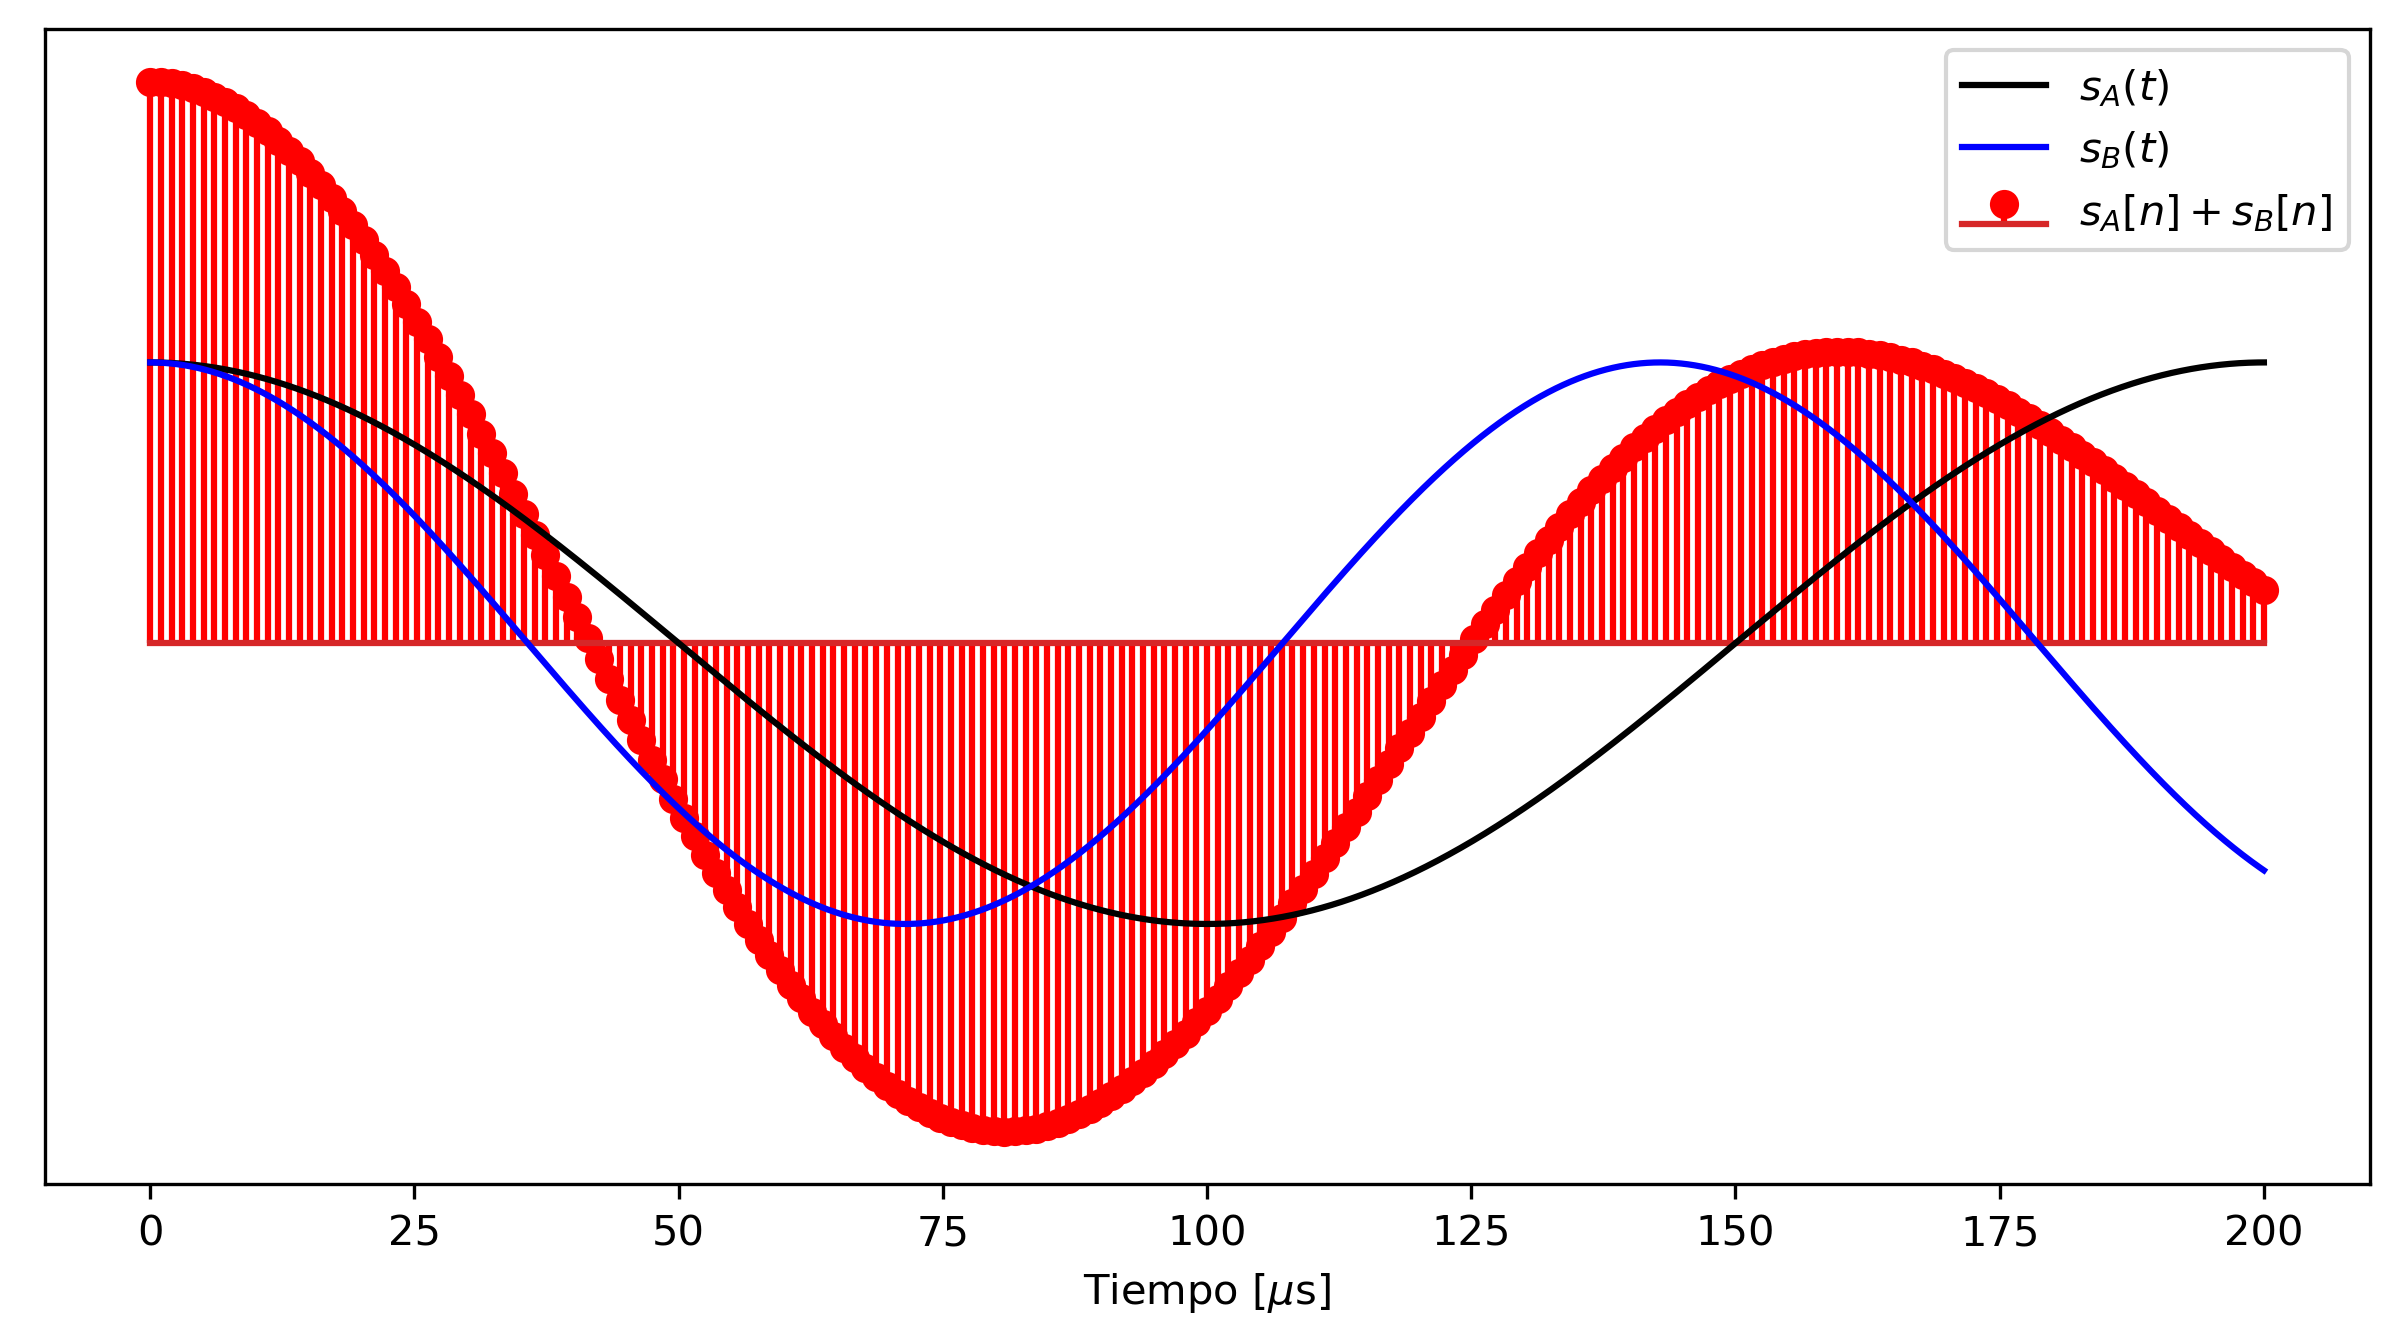
\includegraphics[width=\linewidth]{images/04-Random Sampling/sa_sb.png}
        \caption{$t=[0,200]\; \mu \textrm{s}$}
        \label{fig:rs_sa_sb}
    \end{subfigure}
    \hfill
    \begin{subfigure}[b]{0.9\textwidth}
        \centering
        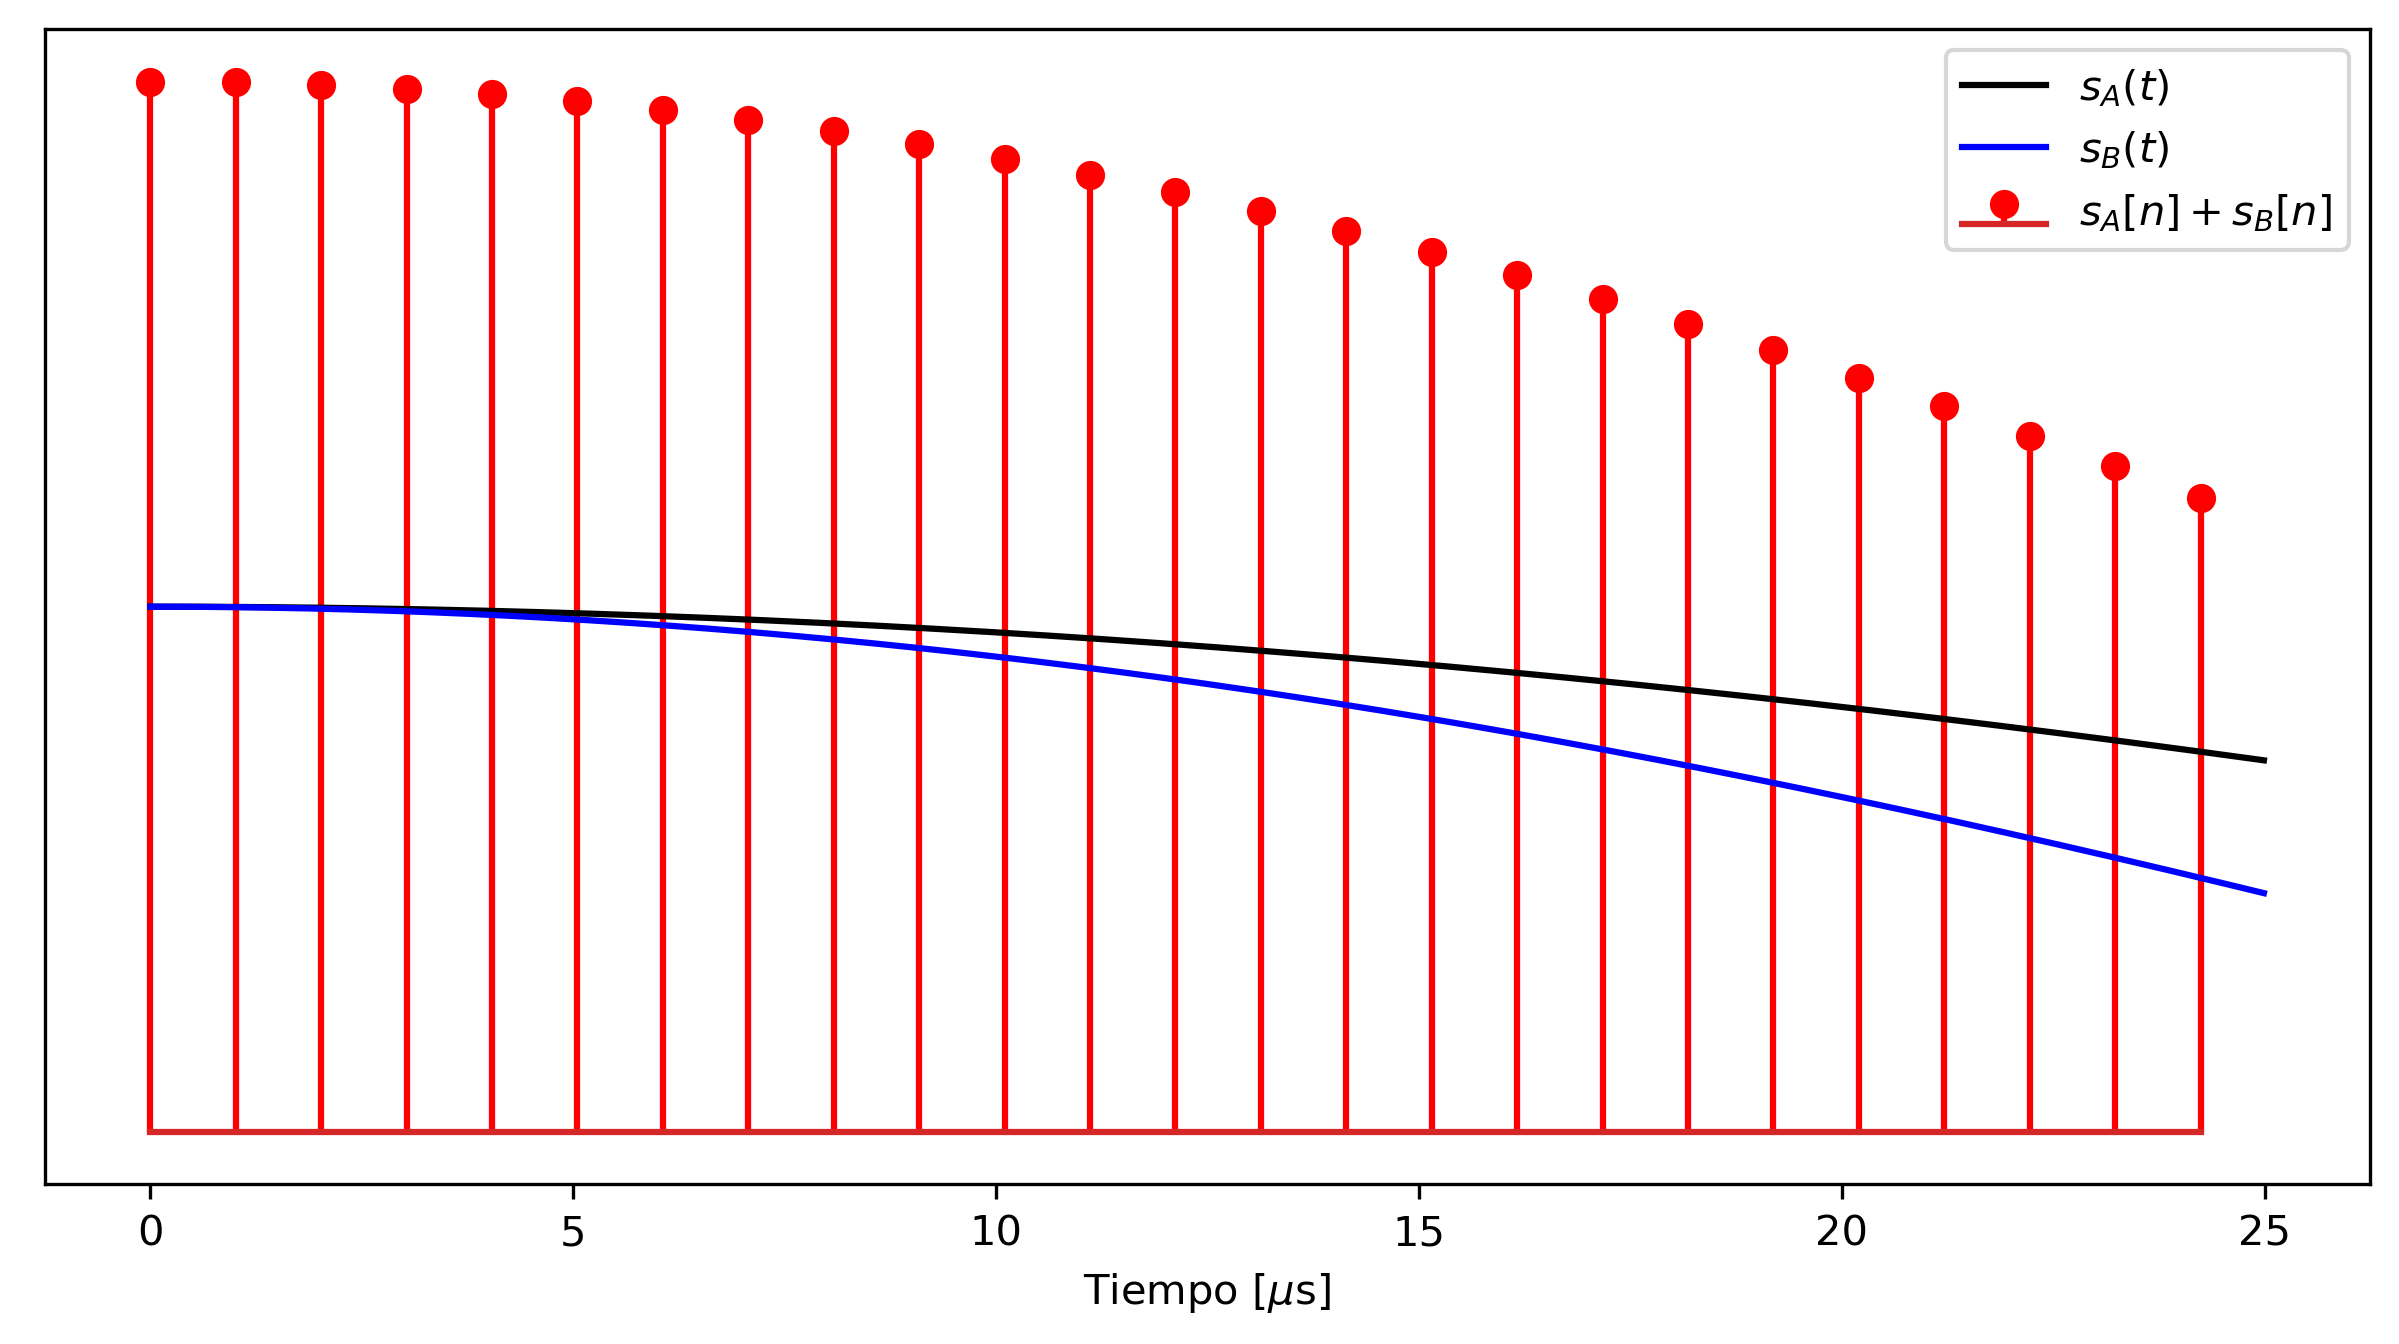
\includegraphics[width=\linewidth]{images/04-Random Sampling/sa_sb_15.png}
        \caption{$t=[0,25]\; \mu \textrm{s}$}
        \label{fig:rs_sa_sb_15}
    \end{subfigure}
    \caption{Señal resultante al muestrear a $f_s=1\textrm{ MHz}$ un elemento de un arreglo de antenas al cual le llegan dos señales senoidales de frecuencias $f_A=5\textrm{ kHz}$ y $f_B={7\textrm{ kHz}}$.}
\end{figure}

Una solución a este problema es reducir la frecuencia de muestreo, de manera tal de obtener mayor información sobre la variación de la señal resultante manteniendo la cantidad de muestras con las que se desea trabajar, pero este enfoque reduce el ancho de banda de las señales que se pueden detectar y reconstruir, debido a lo que enuncia el teorema de Nyquist \cite{bib:nyquist}. Otro enfoque que permite resolver este problema consiste en muestrear la señal recibida utilizando la máxima frecuencia disponible, pero eligiendo aleatoriamente los instantes de muestreo, como se muestra en la Figura \ref{fig:rs_random_sampling_sine}, en la cual se tomaron 25 muestras aleatoriamente a lo largo de 200 $\mu$s. Esta gráfica induce a pensar que estas 25 muestras tomadas en un intervalo de tiempo más separado contienen más información que las muestras de la Figura \ref{fig:rs_sa_sb_15}, y al mismo tiempo se mantiene la frecuencia de muestreo, lo cual permite aplicar el mismo método a señales de mayor ancho de banda \cite{bib:bonetto}.
\begin{figure}[ht!]
    \centering
    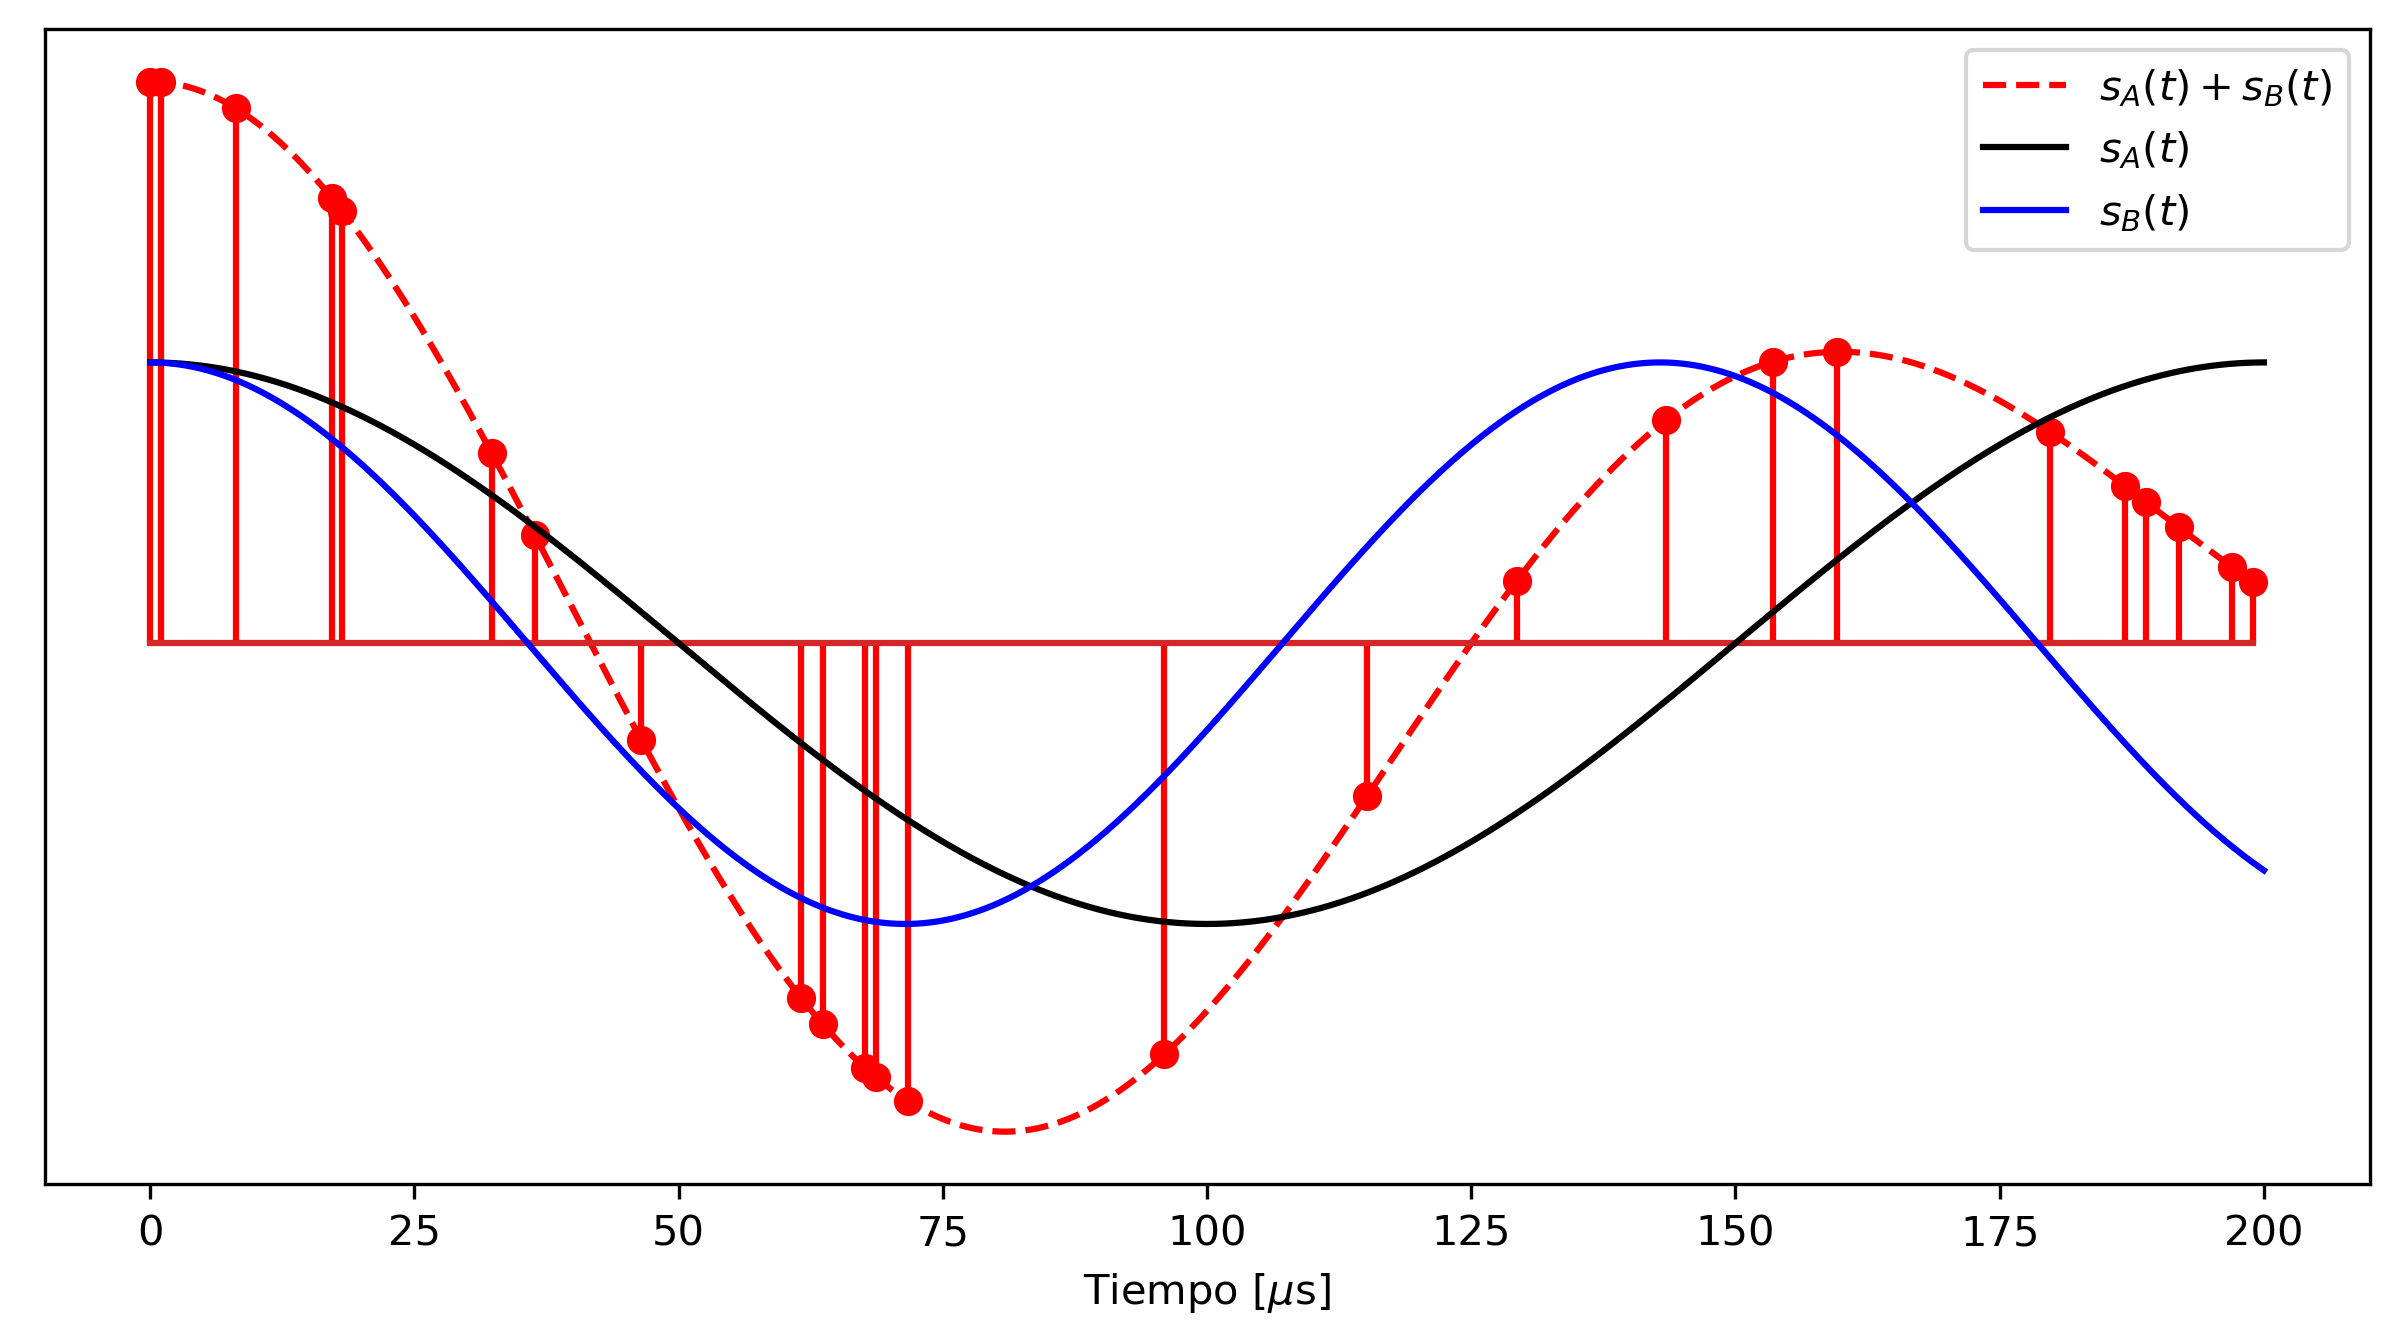
\includegraphics[width=0.9\linewidth]{images/04-Random Sampling/rs_random_sampling_sine.png}
    \caption{Señal resultante al muestrear a $f_s=1\textrm{ MHz}$ un elemento de un arreglo de antenas al cual le llegan dos señales senoidales de frecuencias $f_A=5\textrm{ kHz}$ y $f_B={100\textrm{ kHz}}$ escogiendo 25 muestras utilizando muestreo aleatorio.}
    \label{fig:rs_random_sampling_sine}
\end{figure}

A lo largo de este capítulo se esbozará una justificación teórica de esta propuesta para luego indicar con simulaciones las mejoras alcanzadas.

\section{Definición del problema}\label{subc:rs_problema}

Para resolver el problema de distinguir dos señales dadas $f(t)$ y $g(t)$ puede definirse una buena métrica que viene de la noción geométrica de considerar qué tan ``alienadas'' se encuentra una con respecto a la otra. Esta noción es de especial interés cuando se puede considerar que se trabaja con espacios vectoriales (como lo es el espacio de señal), ya que dicha métrica puede determinarse obteniendo el producto interno entre las señales, el cual está definido como:
\begin{equation}
    \left \langle f,g \right \rangle = \int_{T} f(t) g^*(t)dt,
    \label{eq:rs_prodint}
\end{equation}
siendo T el intervalo temporal en el cual se realiza la integración. Si multiplicamos esta ecuación por $T^{-1}$ tenemos (en el contexto adecuado) un estimador de la correlación cruzada entre dos procesos estocásticos $f$ y $g$, ya que:
\begin{equation}
    \frac{1}{T} \int_{T} f(t) g^*(t)dt = \mathbf{E}[f(t),g(t)]=\mathbf{R}_{f,g}
\end{equation}

De aquí en adelante nos atendremos a la correlación como medida de distinguibilidad de las señales con las que trabajamos.

En lo que sigue vamos a restringir el análisis a señales centradas alrededor de una portadora de frecuencia $\omega_c=2\pi f_c$ y que pueden considerarse de banda angosta, es decir, que su ancho de banda $BW \ll \omega_c$. Luego, para señales de la forma $x(t) = \mathrm{Re}\{a(t) e^{j \omega_c t} \}$, podemos decir que la envolvente compleja $a(t)= \rho(t) e^{j \phi(t)}$, siendo $\rho(t)$ una señal real, es tal que verifica que $\rho(t) \approx \mathrm{cte.}$ para intervalos de tiempo un orden de magnitud mayores al período de la portadora.

Como ejemplo para motivar el resto del análisis, se consideran dos señales $x(t)$ e $y(t)$ de banda angosta, donde $x(t)$ es una referencia nominal contra la que se quiere comparar una señal $y(t)$ recibida. En particular:
\begin{equation}
    \begin{split}
        x(t) & =\mathrm{Re} \{ a(t) e^{j\omega_c t} \} \approx a \cos (\omega_c t)                    \\
        y(t) & =\mathrm{Re} \{ b(t) e^{j(\omega_c t +\phi (t))} \} \approx b \cos (\omega_c t +\phi(t))
    \end{split}
\end{equation}

La correlación cruzada entre $x(t)$ e $y(t)$ viene dada por:
\begin{equation}
    \mathbf{\hat{R}}_{xy}=\frac{1}{T} \int_0 ^T ab \cos(\omega_c t) \cos(\omega_c t + \phi(t))dt
    \label{eq:rs_rxy}
\end{equation}
donde $\phi(t)$ puede ser un desfasaje constante o tener un comportamiento arbitrario en función del tiempo. Se analiza el caso en el que:
\begin{equation}
    \phi(t)\approx\phi_0 + \delta \omega t,
    \label{eq:rs_phi}
\end{equation}
con $\phi_0$ y $\delta \omega$ constantes. Debe notarse que para señales de banda angosta la aproximación de la Ecuación \ref{eq:rs_phi} puede resultar bastante general incluso para tiempos que representen varios períodos de la portadora, y en cuyo caso también valdrá que $\delta \omega \ll \omega_c$. Para tener una intuición del problema que se está planteando, $\phi(t)$ podría estar representando el corrimiento Doppler de una señal recibida respecto a los valores nominales de frecuencia de la portadora.

Sin pérdida de generalidad, se considera $\phi_0=0$, en cuyo caso, la Ecuación \ref{eq:rs_rxy} resulta ser:
\begin{equation}
    \mathbf{\hat{R}}_{xy}= \frac{1}{2} \left[ \mathrm{sinc}(2(2f_c+\delta f)T) + \mathrm{sinc}(2\delta f T) \right] \approx \frac{1}{2} \left[ \mathrm{sinc}(4f_c T) +\mathrm{sinc}(2\delta fT) \right]
    \label{eq:rs_rxyest}
\end{equation}
con $\delta f=\delta \omega /(2\pi)$ y habiendo usado la suposición $\delta f\ll f_c$ para la aproximación. Si se dispone de un tiempo de observación $T$ lo suficientemente grande, la Ecuación \ref{eq:rs_rxyest} dará que la correlación cruzada tiende a cero, y esta es la magnitud que representa la relación de interés entre las dos señales.  Si se considera adicionalmente que $|\mathrm{sinc}(x)|\leq \pi^{-1} \frac{1}{|x|}$ podemos deducir que la condición para obtener la correlación cruzada entre $x(t)$ e $y(t)$ con un error de a lo sumo $\epsilon$ debe ser:
\begin{equation}
    T>\frac{1}{2\pi \delta f \epsilon}
    \label{eq:rs_t_geq}
\end{equation}
donde nuevamente se supuso $\delta f \ll f_c$.

Si ahora se consideran señales de tiempo discreto que representan a las señales de interés muestreadas a una cierta tasa de muestreo $f_s = \frac{1}{T_s}$, entonces se puede aproximar la Ecuación \ref{eq:rs_rxy} haciendo:
\begin{equation}
    \mathbf{\hat{R}_{xy}}:=\frac{1}{N} \sum_{n=0}^{N-1} x(nT_s)y(nT_s)
    \label{eq:rs_rxydisc}
\end{equation}
con $N= \frac{T}{T_s}$.

A esta altura ya se está en condiciones de enunciar el problema que motiva el presente capítulo: por un lado, se desea que la Ecuación \ref{eq:rs_rxydisc} sea una buena aproximación de \ref{eq:rs_rxyest} para un error $\epsilon$ suficientemente pequeño, y por otro, se quiere que la cantidad de muestras $N$ sea lo más pequeña posible para disminuir la carga computacional.

Antes de enunciar la proposición que motiva el presente estudio, se enumeran algunas alternativas \emph{naive} que fueron brevemente mencionadas en la Sección \ref{subc:rs_intro} para intentar dar una solución al problema planteado:
\begin{itemize}
    \item Dado un cierto $T_s$ fijo que hace que la Ecuación \ref{eq:rs_rxydisc} pueda considerarse una buena aproximación de la Ecuación \ref{eq:rs_rxyest} se podría escoger un $N_1<N$, donde $NT_s=T$, pero en este caso no se puede cumplir con condición de la Ecuación \ref{eq:rs_t_geq}. Más aún, de la forma misma que adopta la correlación cruzada, se puede ver que si se achica mucho el número de muestras consideradas, se puede llegar a valores de correlación cruzada que indiquen una considerable correlación entre las señales comparadas, y eso es exactamente lo opuesto a lo que debe manifestarse.
    \item Si se fija el intervalo de integración $T$ se garantiza que se verifica la Ecuación \ref{eq:rs_t_geq} en tiempo continuo, pero para pasar a discreto, si se desea achicar $N$ aparece la obligación de aumentar $T_s$. De este modo la aproximación de la Ecuación \ref{eq:rs_rxydisc} a la Ecuación \ref{eq:rs_rxyest} es el factor limitante, y con la disminución del número de muestras rápidamente se pierde convergencia al valor buscado. Para visualizar esto de un modo intuitivo se puede pensar lo siguiente: si se disminuye la frecuencia de muestreo $f_s$ al punto de dejar de cumplir con el teorema de muestreo de Nyquist \cite{bib:nyquist}, luego se manifestarán en el espectro de la señal discretizada alias correspondientes a frecuencias menores. Como se vio de la Ecuación \ref{eq:rs_rxyest} y la condición de la Ecuación \ref{eq:rs_t_geq}, cuanto menores sean las frecuencias involucradas, el tiempo $T=NT_s$ necesario para poder distinguirlas (es decir, que la correlación cruzada converja a menos del error $\epsilon$) será mayor.
\end{itemize}

Como se vio, disminuir la cantidad de muestras ya sea achicando el intervalo de integración numérica o, si se deja este último fijo, aumentando el tiempo entre muestras, no conduce a los resultados esperados. Intuitivamente, si se quiere achicar la cantidad de muestras pero conservando el intervalo total de observación y al mismo tiempo sin perder información que ocurre a escalas temporales pequeñas, no parece haber alternativa a utilizar algún tipo de de distribución de tiempos entre muestras que no sea uniforme. En particular, como a priori se desea trabajar con señales genéricas, lo que se propone es que esta distribución siga algún tipo de ley aleatoria que no favorezca ninguna escala temporal en particular. Esto lleva a enunciar el algoritmo de \emph{muestreo aleatorio} que se desarrolla en la próxima sección.

Como última observación, cabe destacar que al quitar muestras ocurre que porciones de las señales que se encontraban correlacionadas seguirán correlacionadas mientras que otras que estaban decorrelacionadas no lo estarán más, es por esto que el análisis llevado a cabo se para en este eslabón débil para motivar el método.


\section{Muestreo Aleatorio}\label{subc:rs_muestreoaleatorio}

Teniendo en mente la intuición que surgió de la motivación de la sección anterior, se considera lo que sucede con una versión en tiempo discreto de la señal $z(t)=x(t)y(t)$. Se considera como señal muestreada a:
\begin{equation}
    z_m(t)=z(t)s_m(t),
\end{equation}
donde
\begin{equation}
    s_m(t)=\left( \sum_{n \in \mathbb{Z}} \delta (t-nT_s) \right) m(t)
\end{equation}
y m(t) es una \emph{máscara de muestreo}. Si, por ejemplo, $m(t)=1$ para todo $t$, luego se tiene que $z_m(t)$ se corresponde a $z(t)$ muestreada idealmente y la correlación de la Ecuación \ref{eq:rs_rxydisc} se puede calcular como:
\begin{equation}
    \mathbf{R}_{xy}=\frac{T_s}{T}\int_0^T z_m(t)dt
    \label{eq:rs_rz}
\end{equation}
de forma exacta. Sin embargo, como ya se adelantó, interesa utilizar una forma de muestreo aleatorio que consiste en definir la máscara $m(t)$ como una realización del proceso estocástico definido por:
\begin{equation}
    M(t)=\sum_{n \in \mathbb{Z}} \Pi \left( \frac{t-nT_s}{T_s} \right) \cdot c_n
\end{equation}
siendo
\begin{equation}
    \Pi(t)=\left\{\begin{matrix}
        1 & t\in [0,1)      \\
        0 & \textrm{c.o.c.}
    \end{matrix}\right.,
\end{equation}
y $c_n$ un proceso aleatorio discreto tal que $c_n=1$ con probabilidad $p$, $c_n=0$ con probabilidad $1-p$ y $c_n$ es independiente de $c_m$ para todo $n\neq m$. Nótese que para $p=1$ se está en el caso de muestreo ideal, y para $p=0$ no se utiliza ninguna muestra. El valor esperado de muestras utilizando este enfoque es $pT/T_s$.

La clave está en notar que la correlación que se busca aproximar, es decir la indicada por la Ecuación \ref{eq:rs_rz}, se corresponde a calcular numéricamente el valor medio temporal de la señal $z(t)$  a partir de un instante inicial $t=0$. Es decir, interesa específicamente lo que ocurre con la componente de continua de dicha señal. Por otro lado, dada una realización $m(t)$ del proceso $M(t)$ para una cierta probabilidad $p$, se puede reescribir:
\begin{equation}
    m(t)=\mu_m+m_0(t),
\end{equation}
con $\mu_m$ siendo una constante que representa el valor medio de $m(t)$ y cuyo valor esperado es $p$, y $m_0(t)=m(t)-\mu_m$, siendo $m_0(t)$ una realización del proceso $M(t)-p$, es decir, un proceso con las mismas características que $M(T)$ pero de media nula.

Ahora se está en condiciones de calcular la Ecuación \ref{eq:rs_rz} que comprende el resultado principal de esta propuesta. Esto es:
\begin{equation}
    \frac{T_s}{T}\int_0^T z_m(t)dt = \mu_m \mathbf{R}_{xy} + \frac{T_s}{T} \int_0^T z(t)m_0(t)dt
\end{equation}

El primer término es la correlación que se busca determinar a menos de un factor $\mu_m$ conocido, y el segundo término representa el ``ruido'' que se agrega por la utilización del método de muestreo aleatorio propuesto. Para mayor claridad, si se multiplica por $\mu_m^{-1}$ ambos lados de la igualdad se tiene:
\begin{equation}
    \mu_m^{-1} \left( \frac{T_s}{T} \int_0^T z_m(t)dt \right) = \mathbf{R}_{xy}+\mu_m^{-1} \left(\frac{T_s}{T}  \int_0^T z(t)m_0(t)dt \right),
\end{equation}
lo que deja en evidencia que al disminuir el valor de $\mu_m$ y, por lo tanto, usar menos muestras, también se amplifica el valor del ruido (ya que $0<\mu_m\leq 1$). También se puede estimar con gran precisión cuánto vale ese ruido en la determinación de $\mathbf{R}_{xy}$. Suponiendo que $T_s \ll T$ y que $z(t)$ es independiente de $m_0(t)$, se puede mostrar fácilmente que:
\begin{equation}
    \left| \int_0^T z(t)m_0(t)dt \right| \leq \frac{M_z T_s}{2}
\end{equation}
con $M_z=\mathrm{max}_{0\leq t \leq T} (|z(t)|)$, de modo que el ruido en la estimación de la correlación $\mathbf{R}_{xy}$ por el método de muestreo aleatorio queda acotado por:
\begin{equation}
    \mu_m^{-1} \frac{M_z}{2} \frac{T_s^2}{T}
\end{equation}

A modo de ejemplo, en la Figura \ref{fig:rs_rxy} se presenta el cálculo numérico de la correlación $\mathbf{R}_{xy}$ para señales $x(t)$ e $y(t)$ como las presentadas en la Sección \ref{subc:rs_problema} para $\delta_\omega = \frac{\omega_0}{10}$ y utilizando muestreos aleatorios con distintos valores de $p$. Las funciones de correlación están calculadas para $T$ variando entre 0 y un valor suficientemente grande. Como se puede ver, tanto para $p$ grandes como pequeños la aproximación es muy buena.

\begin{figure}[ht!]
    \centering
    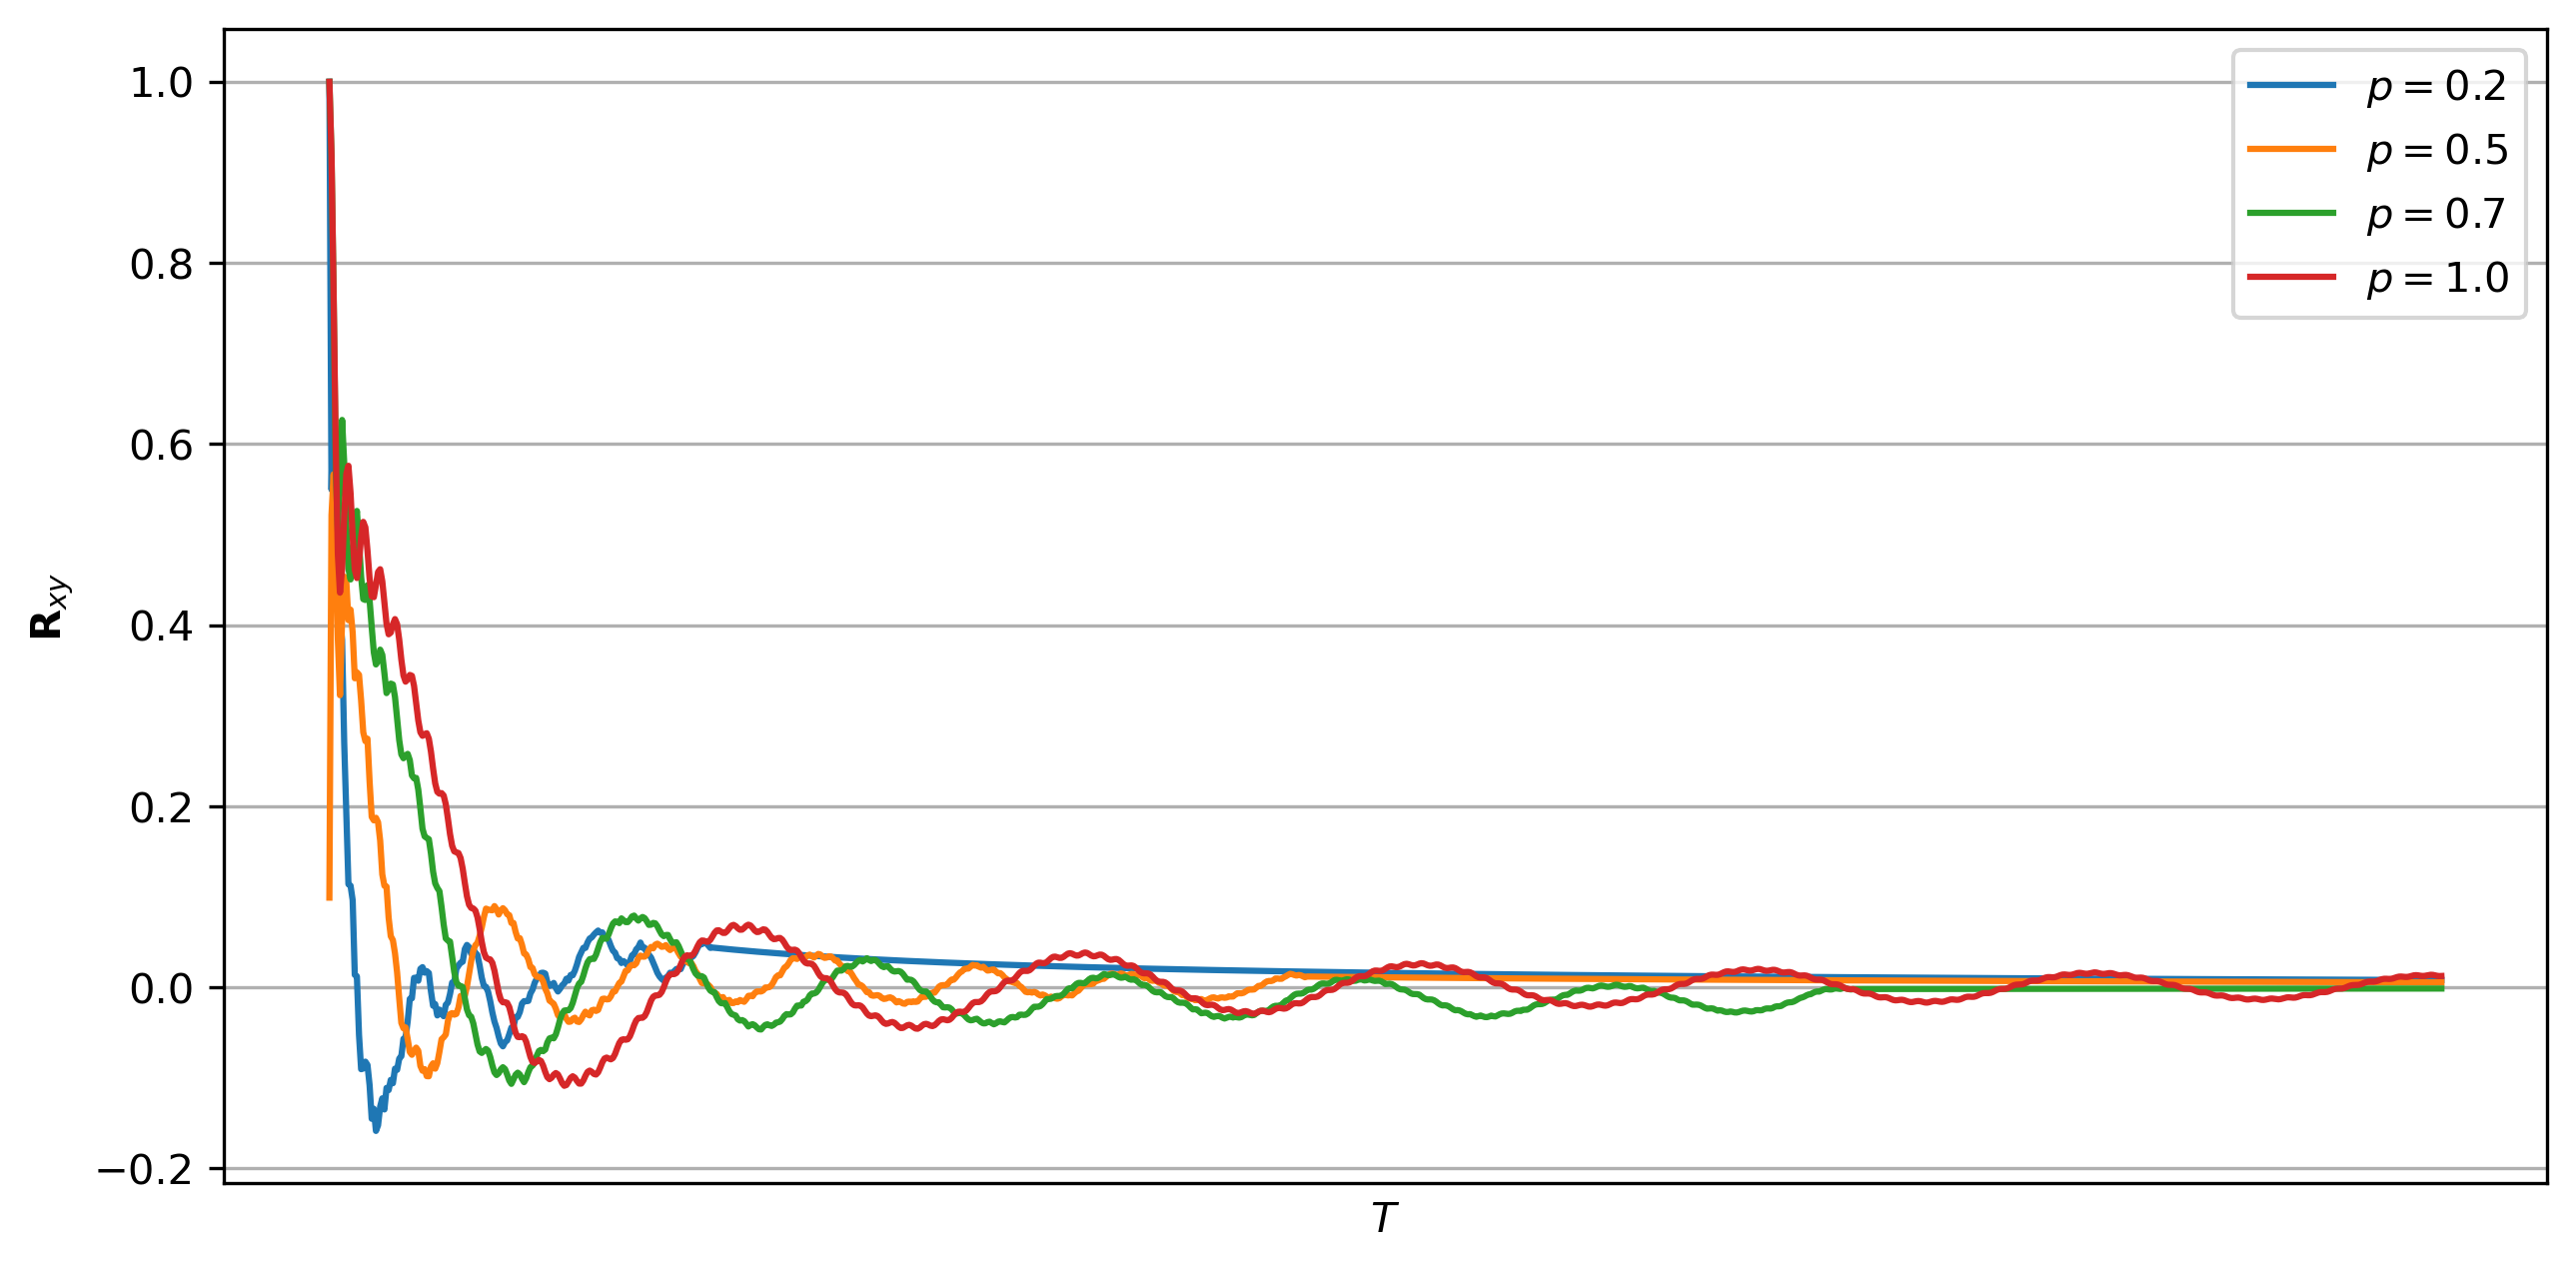
\includegraphics[width=0.9\linewidth]{images/04-Random Sampling/rs_rxy.png}
    \caption{Correlación cruzada entre $x(t)$ e $y(t)$ en función de $T$ utilizando muestreo aleatorio con distintos valores $p$.}
    \label{fig:rs_rxy}
\end{figure}

Finalmente en la Figura \ref{fig:rs_vs_T} se muestra una simulación que se realizó emulando la recepción de beacons muestreados a una frecuencia $f_s=48 \mathrm{ kHz}$ de los satélites GOMX-1 y AISTECHSAT-3 en distintas direcciones y comparando el error obtenido en la estimación utilizando muestreo ideal ($p=1$) con el obtenido utilizando muestreo aleatorio para distintos valores de $p$. Se puede observar que hasta para $p=0,1$, es decir, utilizando el 10\% de las muestras totales, el error obtenido se encuentra en el mismo orden que para el caso de $p=1$. Para el caso de $p=0,01$ el error sube un orden de magnitud con respecto al muestreo secuencial, lo cual tiene sentido ya que se espera que la varianza sea proporcional a la inversa del número de muestras independientes. También se observa cómo el error disminuye a medida que aumenta la ventana de observación $T$. En la práctica habrá que analizar esta relación de compromiso eligiendo valores de $p$ y $T$ que generen un error tolerable y al mismo tiempo permitan tener un tamaño de muestras que puedan ser operables en tiempo real.

\begin{figure}[ht!]
    \centering
    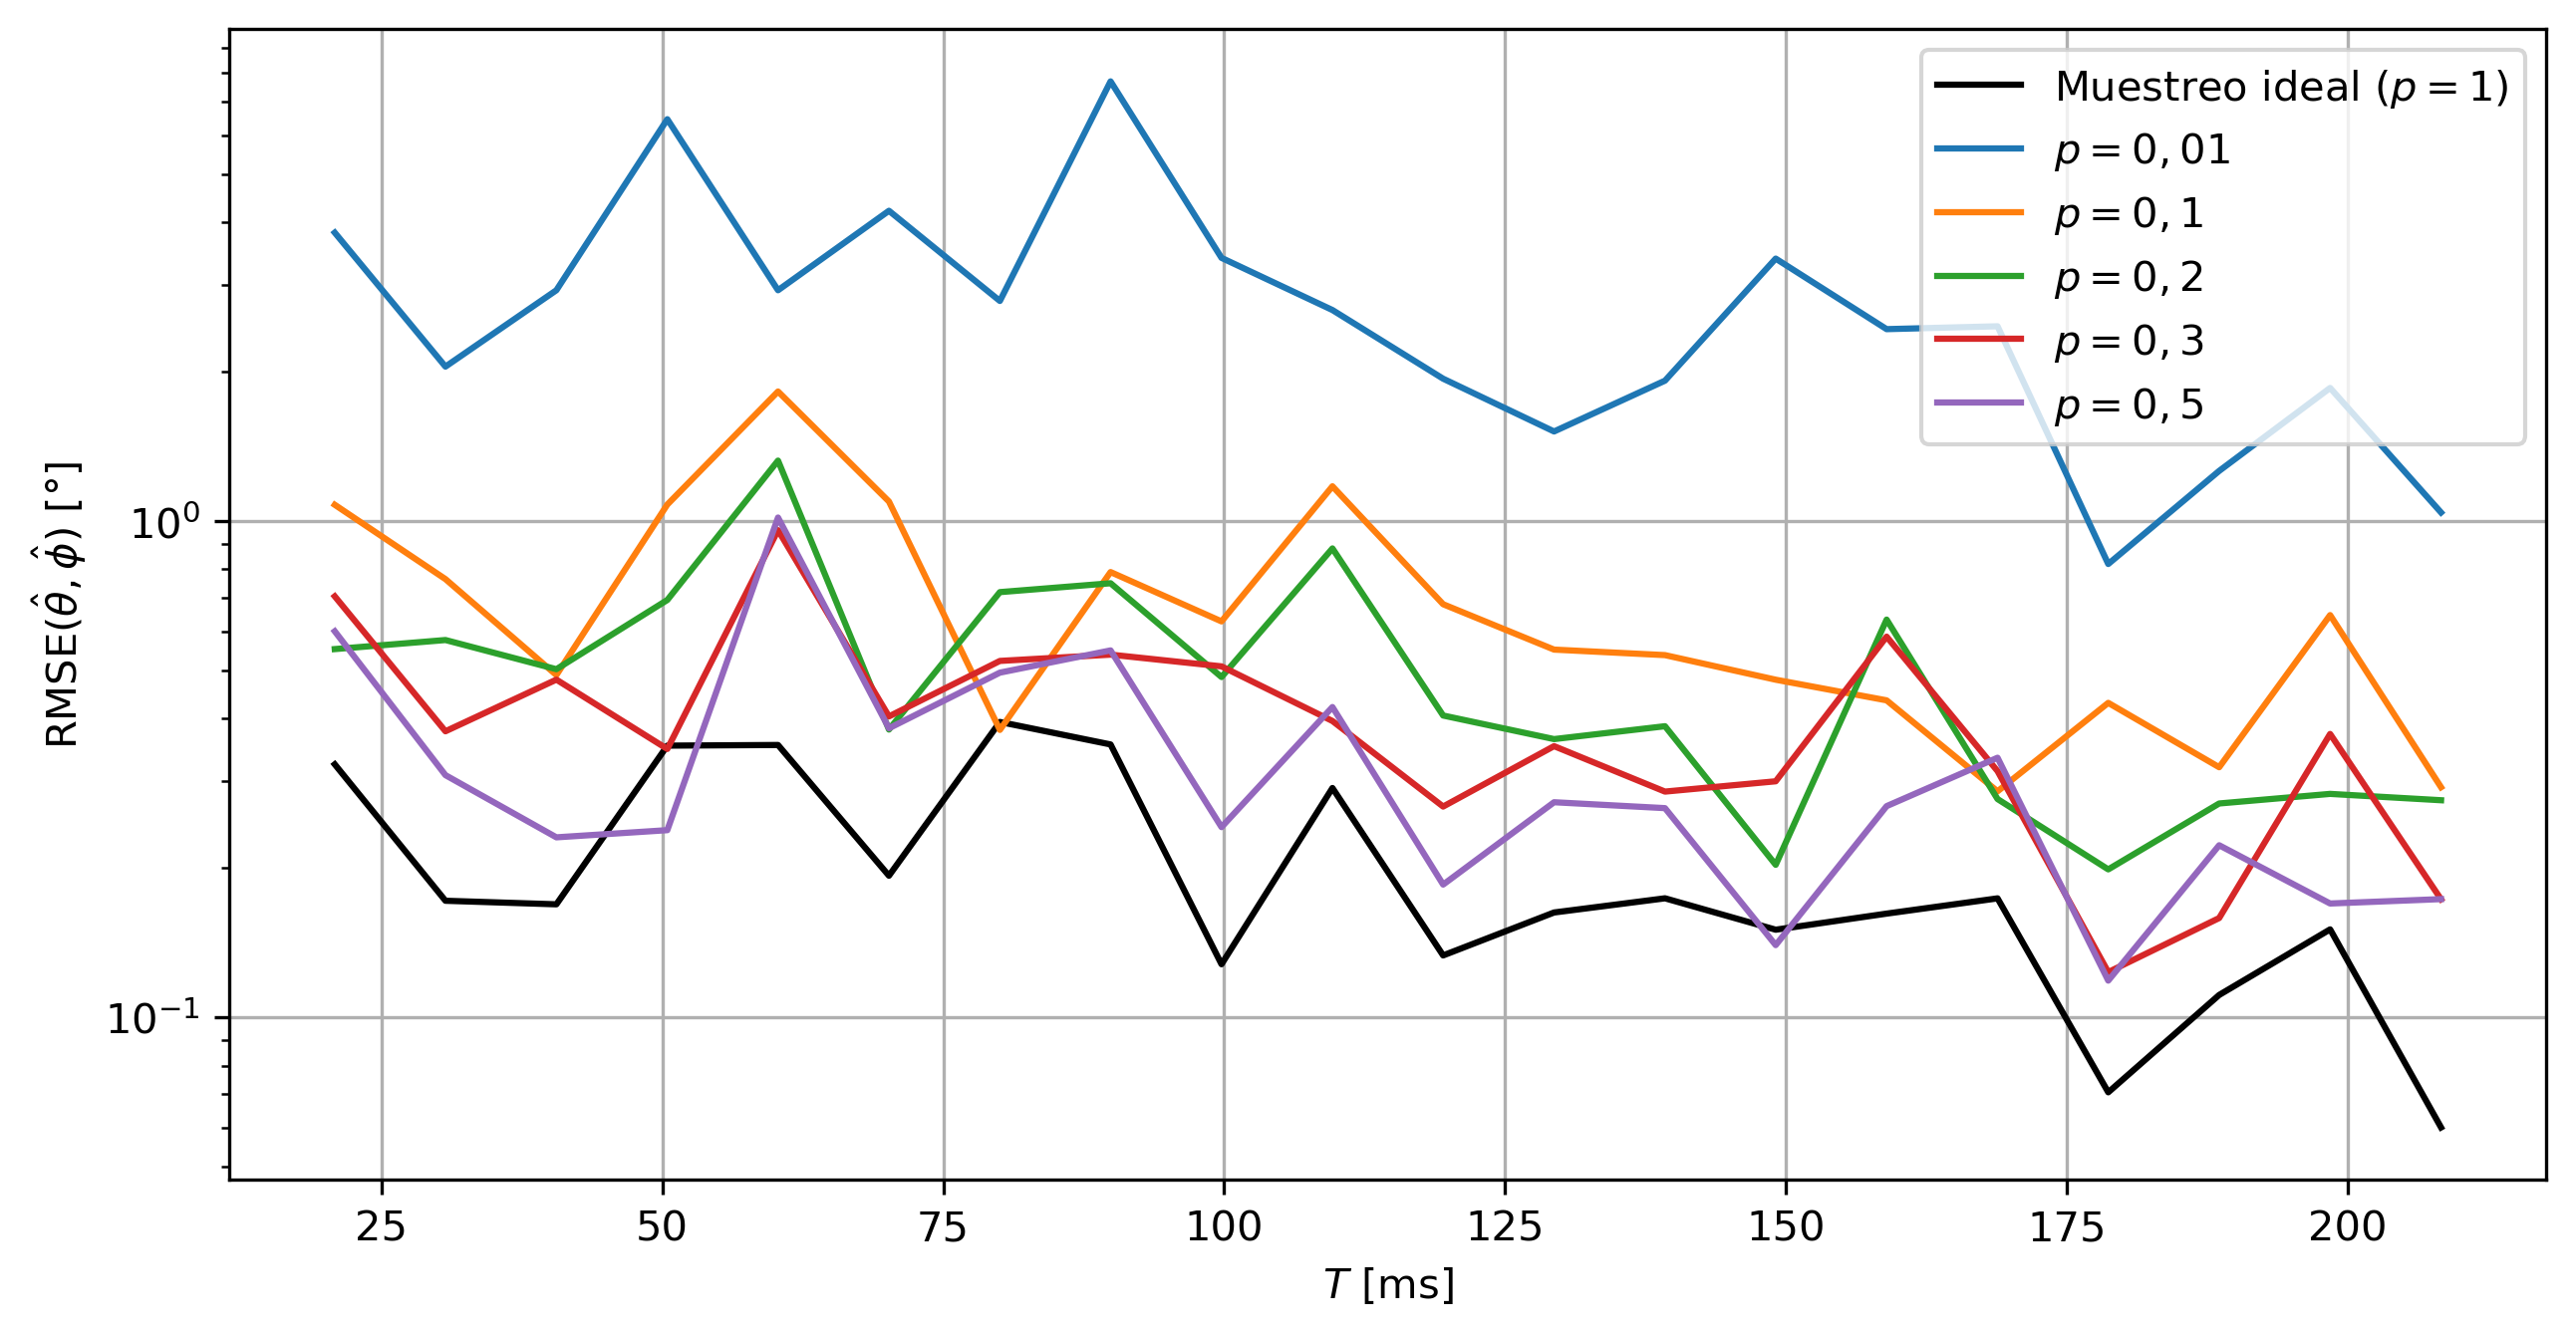
\includegraphics[width=0.9\linewidth]{images/04-Random Sampling/rs_vs_T.png}
    \caption{Gráfica de comparación del RMSE en función de la ventana de observación $T$ para distintos valores de $p$ al recibir dos señales en distintas direcciones.}
    \label{fig:rs_vs_T}
\end{figure}
% music esprit vs N con y sin RS